\documentclass[Lecture.tex]{subfiles}
\begin{document}
\section{5.1: Distance and Accumulated Change}

\subsection{Constant Functions}
\begin{frame}{Constant Functions}
  \only<1-5>{Suppose a car is traveling at 60 miles per hour for 2 hours.
  \onslide<2->{How far did the car go?}\\}
  \vfill
  \begin{minipage}[t]{\linewidth}
    \only<3-5>{
      This is easy:
      $$\onslide<4-5>{60\ \frac{\text{miles}}{\text{hour}} \cdot 2\ \text{hours} =} \onslide<5>{120\ \text{miles}.}$$
    }
    \only<6-7>{
      Geometrically, this is the area under the constant curve $y(t) = 60$ between $t = 0$ and $t = 2$:
      \onslide<7>{\begin{center}
        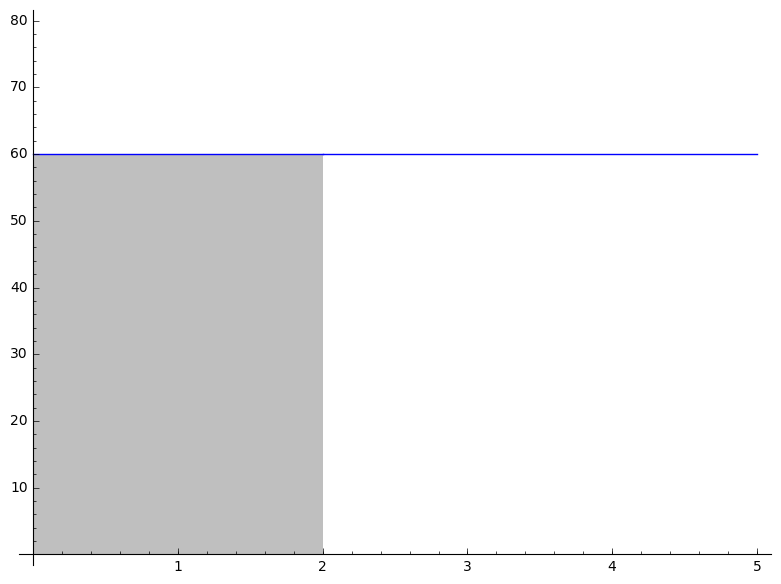
\includegraphics[scale=0.25]{constantVelocity}
      \end{center}}
    }
    \only<8>{
      This says that under constant velocity, $v$, the position of the car, $s(t)$, relative to the starting point at time $0 \leq t$ is just
      $$s(t) = v \cdot t.$$
    }
  \end{minipage}
\end{frame}

\subsection{Linear Functions}
\begin{frame}{Linear Functions}
  \only<1-3>{According to Car and Driver, a 2006 Bugatti Veyron is capable of an acceleration of $11.59 \operatorname{m}/\operatorname{s}^2$.
  Assume the car starts at rest and accelerates at this constant rate.\\}

  \vfill
  
  \begin{minipage}[t]{\linewidth}
    \only<2-3>{
      By the observation in the last example, we can compute the velocity at time $t$ as the area under the constant curve $y(t) = 11.59$:
      \onslide<3>{
        \begin{center}
          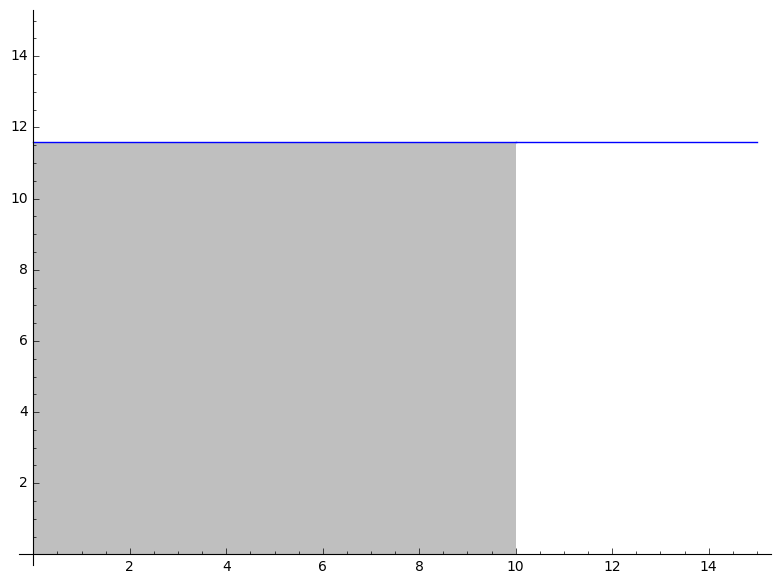
\includegraphics[scale=0.25]{constantAcceleration}
        \end{center}
      }
    }
    \only<4-5>{
      The velocity is linear: $v(t) = 11.59\cdot t$.
      Hence the position, $s(t)$, is the area under the velocity curve:
      \onslide<5->{
        \begin{center}
          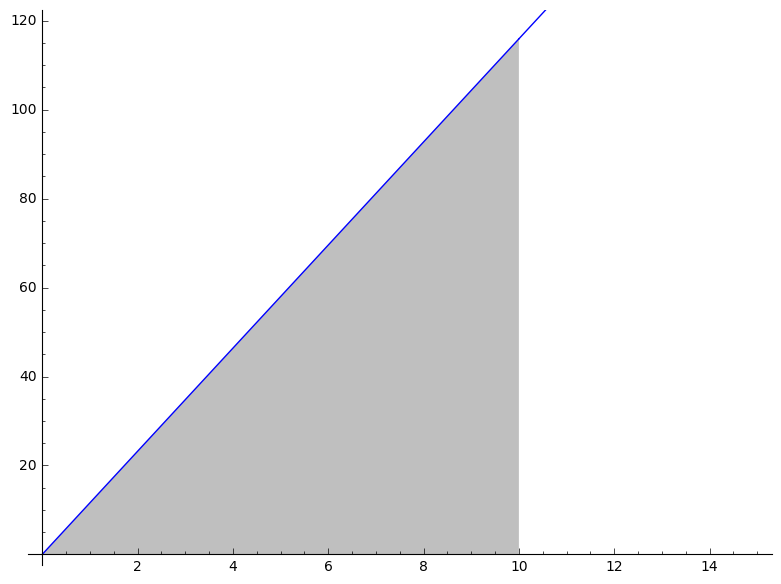
\includegraphics[scale=0.25]{linearVelocity}
        \end{center}
      }
    }
    \only<6->{
      Therefore the position at time $t$ is:
        \begin{eqnarray*}
          \onslide<7->{s(t) &=&} \onslide<8->{\frac{1}{2}v(t)\cdot t\\} 
          \onslide<9->{ &=& \frac{1}{2}(11.59 \cdot t)\cdot t\\}
          \onslide<10->{ &=& \frac{11.59}{2}t^2.}
        \end{eqnarray*}
      }
  \end{minipage}
\end{frame}

\subsection{Non-Linear Functions}
\begin{frame}{Non-Linear Functions}
  \only<1-12>{What happens when the area is not a nice geometric object?\\}
  \vfill
  \begin{minipage}[t]{\linewidth}
    \only<2-9>{
      Can we tell how far a car traveled if we are given the following table of times and velocities?
      \onslide<3->{
        \begin{center}
          \begin{tabular}{c||c|c|c|c|c|c}
            time (sec) & 0 & 2 & 4 & 6 & 8 & 10\\
            \hline
            speed (ft/sec) & 20 & 30 & 38 & 44 & 48 & 50\\
          \end{tabular}
        \end{center}
      }
      \onslide<4->{This is clearly not linear:}
      \onslide<5->{
        $$\onslide<5->{\frac{30 - 20}{2 - 0} =} \onslide<6->{5}\onslide<7->{\ \text{and}\ }\onslide<8->{\frac{50-48}{10-8}}\onslide<9->{ = 1.}$$
        }
    }
    \only<10-12>{
      We can fit a curve to these points:
      \onslide<11-12>{
        \begin{center}
          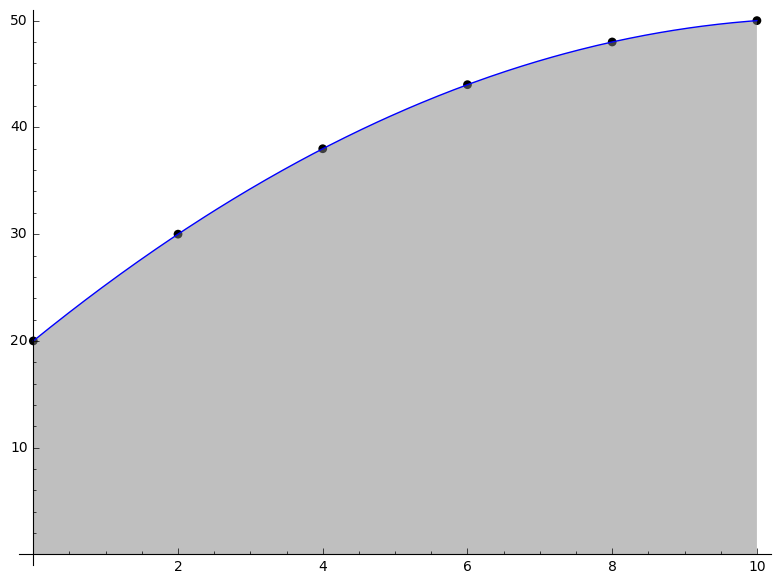
\includegraphics[scale=0.3]{nonlinearVelocity}
        \end{center}
      }
      \onslide<12>{How do we compute the area of the shaded region?}
    }
    \only<13-16>{
      We could assume constant velocity between the two points and estimate.
      \onslide<14->{Say we assume the velocity is the velocity at the left endpoint:}
      \onslide<15->{
        \begin{center}
          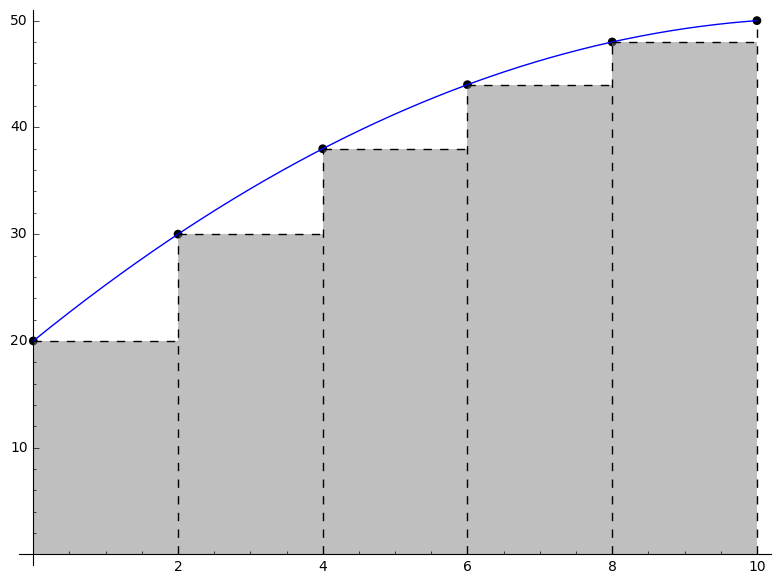
\includegraphics[scale=0.3]{nonlinearLeftSum}
        \end{center}
      }
      \onslide<16->{This is an underestimate of the area.}
    }
    \only<17-22>{
      \begin{center}
          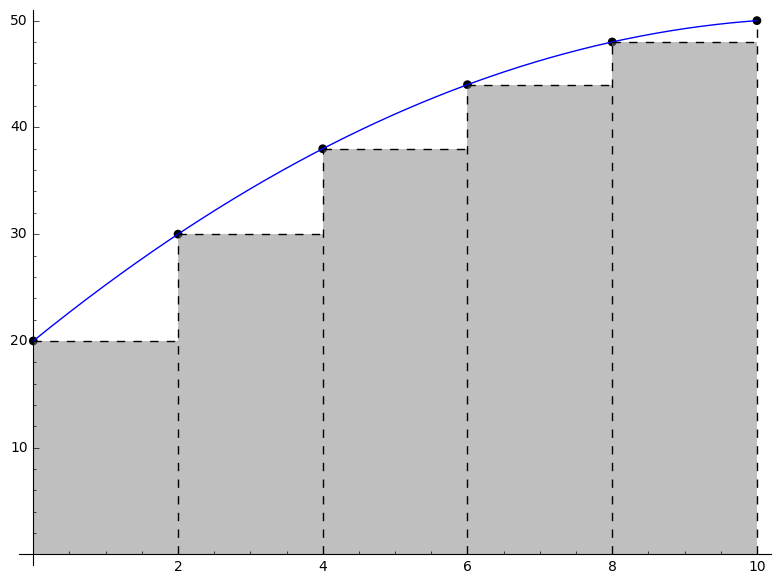
\includegraphics[scale=0.2]{nonlinearLeftSum}
        \end{center}
      
      \begin{itemize}
        \item<17->
          Each rectangle has width 2.
        \item<18->
          The height of each rectangle is the height of the left endpoint.
        \item<19->
          Our area estimate is:
          \begin{eqnarray*}
            \onslide<20->{2(20 + 30 + 38 + 44 + 48) &=&}
            \onslide<21->{2(180)\\}
            \onslide<22->{&=& 360\ \text{feet}.}
          \end{eqnarray*}
      \end{itemize}
    }
    \only<23-25>{
      We could also assume the velocity is the velocity at the right endpoint:
      \onslide<24->{
      \begin{center}
        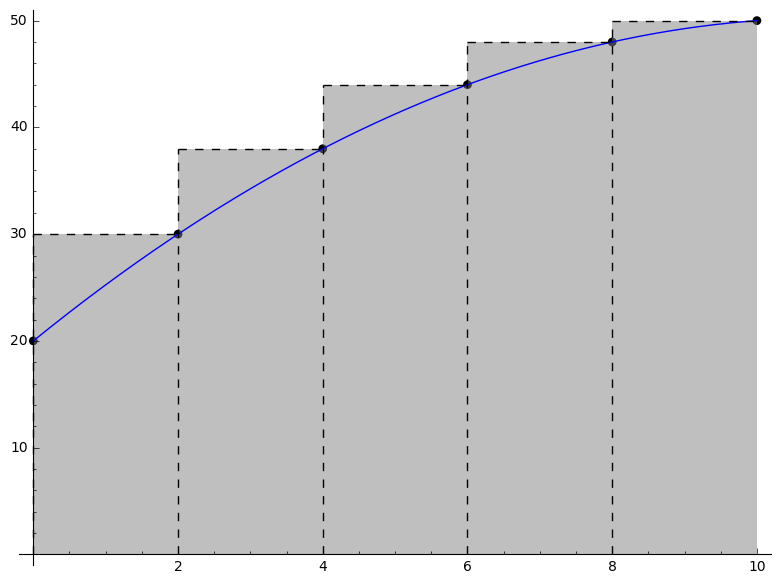
\includegraphics[scale=0.3]{nonlinearRightSum}
      \end{center}
      }
      \onslide<25->{This is an overestimate of the area.}
      }
    \only<26-31>{
      \begin{center}
        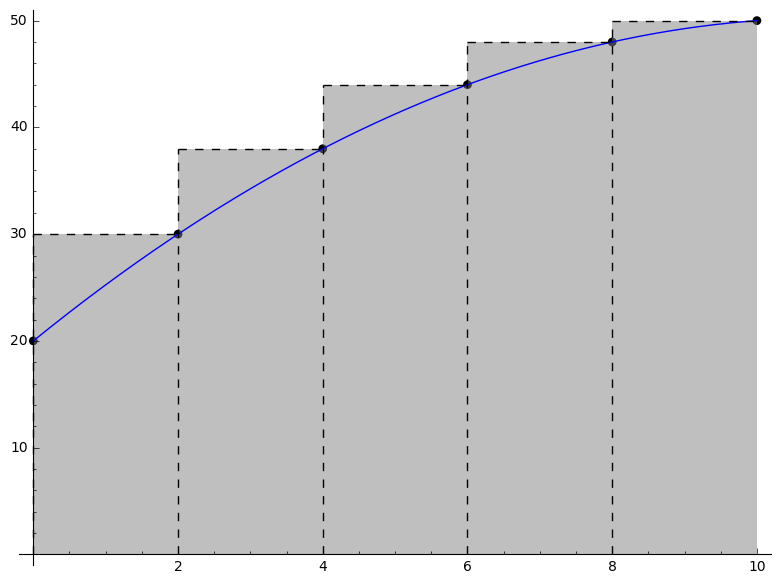
\includegraphics[scale=0.2]{nonlinearRightSum}
      \end{center}
      \begin{itemize}
      \item<26->
        Each rectangle has width 2.
      \item<27->
        The height of each rectangle is the height of the right endpoint.
      \item<28->
        Our area estimate is:
        \begin{eqnarray*}
          \onslide<29->{2(30 + 38 + 44 + 48 + 50) &=&}
          \onslide<30->{2(210)\\}
          \onslide<31->{&=& 420\ \text{feet}.}
        \end{eqnarray*}
      \end{itemize}
    }
    \only<31->{
      This tells us:
      \begin{itemize}
        \item<32->
          The distance traveled is {\bf at least} 360 feet.
        \item<33->
          The distance traveled is {\bf at most} 420 feet.
        \item<34->
          The distance traveled must be somewhere between these two.
        \item<35->
          The average of these estimates is 
          $$\frac{420 + 360}{2} = 390$$
          feet, which gives a better estimate.
      \end{itemize}
      \onslide<36->{Can we do better?}
      \onslide<37->{If so, how?}
    }
  \end{minipage}
\end{frame}
\end{document}
